% Start of user code protected header
\documentclass{gemoc} %% no option needed, default is : 10pt, twoside, babel[ english] , graphicx
\usepackage{color}
\usepackage[colorlinks=true]{hyperref}

\task{x.x.x}
\title{Gemoc XXX }
\docnumber{Dx.x.x}
\version{1.0}

\companycopyright{Consortium GEMOC}  %% Appear in the foot page

\begin{document}
\maketitle

\begin{revisions}
	\begin{revtable}
		\dates{}{}{}{}{}
		\writers{}{}{}{}{}
		\approvers{}{}{}{}{}
	\end{revtable}
	\begin{revisionlabels}
		\revlabel{}
	\end{revisionlabels}
\end{revisions}
\begin{tableofauthors}
	\leadauthor{Didier Vojtisek}{INRIA}
	\contributor{$<$Name$>$}{$<$Organisation$>$}
\end{tableofauthors}

\tableofcontents
\newpage

\chapter{Gemoc language workbench workflow}

%End of user code
%Start of user code summary
The figure \ref{fig:Gemoc_language_workbench_workflow} presents the global view of the workflow of the different activities of the Language Workbench.


In further sections each activity will be detailled by also presenting the major concrete artefacts resulting from the Commands.
%End of user code
\begin{figure}[h!]
		\center
		\includegraphics*[trim=0.0cm 0.0cm 0cm 0.0cm, clip=true]{fig/Gemoc_language_workbench_workflow}
		\caption{Gemoc Language Workbench workflow activities and supported tools}
		\label{fig:Gemoc_language_workbench_workflow}
\end{figure}

% Start of user code protected summary_legend
Legend:
\begin{itemize}
	\item 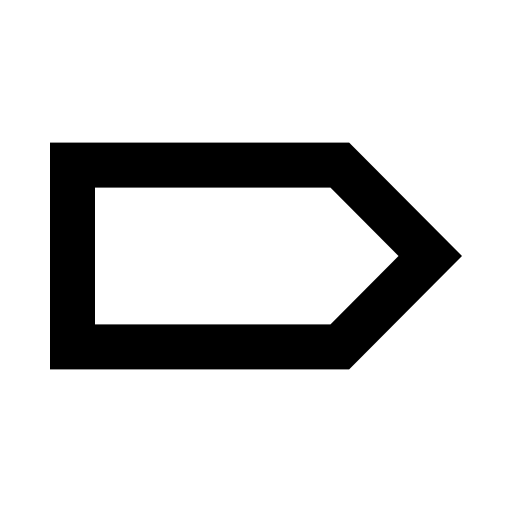
\includegraphics[width=1cm]{fig/step} Activity: an activity is a step of the workflow. Each activity is supported by at least one concrete Command
	\item \includegraphics[width=0.7cm]{fig/command} Command: a command is a concrete action of the studio, usually implemented as a wizard.
	\item \includegraphics[width=0.5cm]{fig/artifact_add} Artifact creation: Artifact created as the result of a command.
	\item \includegraphics[width=0.5cm]{fig/artifact_update} Artifact update:  Artifact updated as the result of a command.
\end{itemize}
%End of user code
\section{xDSML definition}
%%%%%%%%%%%%%%%%%%%%%%%%%%%%%%%%%%%%%%%%%%%%%%%%%%%%%%%
\label{sec:xDSML_definition}
% Start of user code protected xDSML definition
%End of user code
\begin{figure}[h!]
		\center
		\includegraphics*[trim=0.0cm 0.0cm 0cm 0.0cm, clip=true]{fig/xDSML_definition}
		\caption{xDSML definition activity}
		\label{fig:xDSML_definition}
\end{figure}

TODO

The figure \ref{fig:xDSML_definition} presents the activity and its supporting Commands.

\subsection{New GEMOC Language project Command}
TODO
\subsubsection{Created artefacts}
Artifacts created by the New GEMOC Language project Command:
\paragraph{Language workbench project} 
TODO\paragraph{xdsml file} 
TODO
\subsubsection{Updated artefacts}
Artifacts updated by the New GEMOC Language project Command:

	None

\section{Domain Model definition (AS)}
%%%%%%%%%%%%%%%%%%%%%%%%%%%%%%%%%%%%%%%%%%%%%%%%%%%%%%%
\label{sec:Domain_Model_definition__AS_}
% Start of user code protected Domain Model definition (AS)
%End of user code
\begin{figure}[h!]
		\center
		\includegraphics*[trim=0.0cm 0.0cm 0cm 0.0cm, clip=true]{fig/Domain_Model_definition__AS_}
		\caption{Domain Model definition (AS) activity}
		\label{fig:Domain_Model_definition__AS_}
\end{figure}

TODO

The figure \ref{fig:Domain_Model_definition__AS_} presents the activity and its supporting Commands.

\subsection{Create EMF Project Command}
TODO
\subsubsection{Created artefacts}
Artifacts created by the Create EMF Project Command:
\paragraph{EMF project} 
TODO\paragraph{ecore} 
TODO\paragraph{genmodel} 
TODO
\subsubsection{Updated artefacts}
Artifacts updated by the Create EMF Project Command:
\paragraph{xdsml} 
TODO

\subsection{Select existing EMF project Command}

\subsubsection{Created artefacts}
Artifacts created by the Select existing EMF project Command:

	None
\subsubsection{Updated artefacts}
Artifacts updated by the Select existing EMF project Command:
\paragraph{xdsml} 


\section{Modelers definition (CS)}
%%%%%%%%%%%%%%%%%%%%%%%%%%%%%%%%%%%%%%%%%%%%%%%%%%%%%%%
\label{sec:Modelers_definition__CS_}
% Start of user code protected Modelers definition (CS)
%End of user code
\begin{figure}[h!]
		\center
		\includegraphics*[trim=0.0cm 0.0cm 0cm 0.0cm, clip=true]{fig/Modelers_definition__CS_}
		\caption{Modelers definition (CS) activity}
		\label{fig:Modelers_definition__CS_}
\end{figure}

TODO

The figure \ref{fig:Modelers_definition__CS_} presents the activity and its supporting Commands.

\subsection{Select existing Tree editor Command}

\subsubsection{Created artefacts}
Artifacts created by the Select existing Tree editor Command:

	None
\subsubsection{Updated artefacts}
Artifacts updated by the Select existing Tree editor Command:
\paragraph{xdsml} 


\subsection{New Tree editor Command}
TODO
\subsubsection{Created artefacts}
Artifacts created by the New Tree editor Command:
\paragraph{Edit project} 
TODO\paragraph{Editor project} 
TODO
\subsubsection{Updated artefacts}
Artifacts updated by the New Tree editor Command:
\paragraph{xdsml} 
TODO

\subsection{New Xtext editor Command}
TODO
\subsubsection{Created artefacts}
Artifacts created by the New Xtext editor Command:
\paragraph{Xtext project} 
TODO\paragraph{Xtext.ui project} 
TODO
\subsubsection{Updated artefacts}
Artifacts updated by the New Xtext editor Command:
\paragraph{xdsml} 
TODO

\subsection{Select existing Xtext editor Command}

\subsubsection{Created artefacts}
Artifacts created by the Select existing Xtext editor Command:

	None
\subsubsection{Updated artefacts}
Artifacts updated by the Select existing Xtext editor Command:
\paragraph{xdsml} 


\subsection{Select existing Sirius editor Command}

\subsubsection{Created artefacts}
Artifacts created by the Select existing Sirius editor Command:

	None
\subsubsection{Updated artefacts}
Artifacts updated by the Select existing Sirius editor Command:
\paragraph{xdsml} 


\subsection{New Sirius editor Command}
TODO
\subsubsection{Created artefacts}
Artifacts created by the New Sirius editor Command:
\paragraph{Sirius specification project} 
TODO
\subsubsection{Updated artefacts}
Artifacts updated by the New Sirius editor Command:
\paragraph{xdsml} 
TODO

\section{Execution Function and Data definition (DSA)}
%%%%%%%%%%%%%%%%%%%%%%%%%%%%%%%%%%%%%%%%%%%%%%%%%%%%%%%
\label{sec:Execution_Function_and_Data_definition__DSA_}
% Start of user code protected Execution Function and Data definition (DSA)
%End of user code
\begin{figure}[h!]
		\center
		\includegraphics*[trim=0.0cm 0.0cm 0cm 0.0cm, clip=true]{fig/Execution_Function_and_Data_definition__DSA_}
		\caption{Execution Function and Data definition (DSA) activity}
		\label{fig:Execution_Function_and_Data_definition__DSA_}
\end{figure}

TODO

The figure \ref{fig:Execution_Function_and_Data_definition__DSA_} presents the activity and its supporting Commands.

\subsection{New Kermeta 3 project Command}
TODO
\subsubsection{Created artefacts}
Artifacts created by the New Kermeta 3 project Command:
\paragraph{K3 project} 
TODO
\subsubsection{Updated artefacts}
Artifacts updated by the New Kermeta 3 project Command:
\paragraph{xdsml} 
TODO

\subsection{Select existing Kermeta 3 project Command}

\subsubsection{Created artefacts}
Artifacts created by the Select existing Kermeta 3 project Command:

	None
\subsubsection{Updated artefacts}
Artifacts updated by the Select existing Kermeta 3 project Command:
\paragraph{xdsml} 


\section{Concurrency Model definition (MoCC)}
%%%%%%%%%%%%%%%%%%%%%%%%%%%%%%%%%%%%%%%%%%%%%%%%%%%%%%%
\label{sec:Concurrency_Model_definition__MoCC_}
% Start of user code protected Concurrency Model definition (MoCC)
%End of user code
\begin{figure}[h!]
		\center
		\includegraphics*[trim=0.0cm 0.0cm 0cm 0.0cm, clip=true]{fig/Concurrency_Model_definition__MoCC_}
		\caption{Concurrency Model definition (MoCC) activity}
		\label{fig:Concurrency_Model_definition__MoCC_}
\end{figure}

TODO

The figure \ref{fig:Concurrency_Model_definition__MoCC_} presents the activity and its supporting Commands.

\subsection{New MoCCML project Command}

\subsubsection{Created artefacts}
Artifacts created by the New MoCCML project Command:
\paragraph{moccml/ccslLib file} 
\paragraph{eclipse plugin project} 

\subsubsection{Updated artefacts}
Artifacts updated by the New MoCCML project Command:
\paragraph{xdsml} 


\subsection{Select existing MoCCML project Command}

\subsubsection{Created artefacts}
Artifacts created by the Select existing MoCCML project Command:

	None
\subsubsection{Updated artefacts}
Artifacts updated by the Select existing MoCCML project Command:
\paragraph{xdsml} 


\section{Behavioral observation definition (DSE)}
%%%%%%%%%%%%%%%%%%%%%%%%%%%%%%%%%%%%%%%%%%%%%%%%%%%%%%%
\label{sec:Behavioral_observation_definition__DSE_}
% Start of user code protected Behavioral observation definition (DSE)
%End of user code
\begin{figure}[h!]
		\center
		\includegraphics*[trim=0.0cm 0.0cm 0cm 0.0cm, clip=true]{fig/Behavioral_observation_definition__DSE_}
		\caption{Behavioral observation definition (DSE) activity}
		\label{fig:Behavioral_observation_definition__DSE_}
\end{figure}

TODO

The figure \ref{fig:Behavioral_observation_definition__DSE_} presents the activity and its supporting Commands.

\subsection{New ECL file Command}
TODO
\subsubsection{Created artefacts}
Artifacts created by the New ECL file Command:
\paragraph{ecl file} 
TODO
\subsubsection{Updated artefacts}
Artifacts updated by the New ECL file Command:
\paragraph{xdsml} 
TODO

\subsection{New Modelh'x project Command}
TODO
\subsubsection{Created artefacts}
Artifacts created by the New Modelh'x project Command:

	None
\subsubsection{Updated artefacts}
Artifacts updated by the New Modelh'x project Command:

	None

\subsection{Select existing ECL project Command}

\subsubsection{Created artefacts}
Artifacts created by the Select existing ECL project Command:

	None
\subsubsection{Updated artefacts}
Artifacts updated by the Select existing ECL project Command:
\paragraph{xdsml} 


\section{Animators definition}
%%%%%%%%%%%%%%%%%%%%%%%%%%%%%%%%%%%%%%%%%%%%%%%%%%%%%%%
\label{sec:Animators_definition}
% Start of user code protected Animators definition
%End of user code
\begin{figure}[h!]
		\center
		\includegraphics*[trim=0.0cm 0.0cm 0cm 0.0cm, clip=true]{fig/Animators_definition}
		\caption{Animators definition activity}
		\label{fig:Animators_definition}
\end{figure}

TODO

The figure \ref{fig:Animators_definition} presents the activity and its supporting Commands.


%Start of user code protected footer
\end{document}
%End of user code
